%!TEX root = pixel-wise-street-segmentation.tex

\section{Used models}\label{sec:model}

We have implemented two approaches to tackle  the street segmentation problem.
We have used a sliding window approach which is based on a classification
network and a regression approach. Both models are detailed in the following
section.

\subsection{The Sliding Window Approach}
Traditionally neural networks are used for classification tasks. As
described in \cref{sec:related-work} they deliver impressive results. Our first
approach is a sliding window model, which exploits the classification strength
of deep neural networks.

\subsubsection{Definition of the Classification Problem}
We trained a neural network to solve the following binary classification
problem:

\fbox{
    \begin{tabular}{l l}
        \multicolumn{2}{l}{\textbf{Classification Problem}} \\
        \textit{Input:} & A $n \times n$ 3-channel pixel image section.\\
        \textit{Output:} & Decide whether the center pixel is street.
    \end{tabular}
}

For $n$ we used $51$. This constant was chosen as we ran into GPU memory
problems when training on higher values of $n$. Our classification approach is
visualized in \cref{fig:figure}.

\begin{figure}[H]
    \centering
    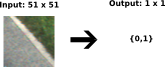
\includegraphics[width=0.5\columnwidth]{figures/models/sliding_window.png}
    \caption{Visualization of the classification problem solved by our neural network.}%
\label{fig:figure}
\end{figure}


\subsubsection{Net Topology}
The problem defined above can be tackled with any of the well known
classification networks such as GoogLeNet or AlexNet. For our solution we
designed our own network detailed in \cref{tab:topo}. The small size of only
three hidden layers was chosen as our experiments showed that small networks
perform better than networks with more layers. One reason for this is that the
amount of labeled images is rather small. Hence smaller nets generalize much
better. Secondly, the binary decision task of recognizing street is much
simpler than detailed image classification. This simplicity does also reflect
in the net topology.

\begin{table}[H]
    \normalsize
    \centering
\begin{tabular}{r  l l}
    \toprule
    \textbf{Layer} & \textbf{Type}  & \textbf{Shape}  \\
    \midrule
    0     & Input &  $51 \times 51 \times 3$ \\
    1     & Convolution & 10 filter  each $5 \times 5$ \\
    2     & Convolution & 10 filter  each $5 \times 5$  \\
    3     & Pooling     & $2 \times 2$ \\
    4     & Output     & $1$ \\
    \bottomrule
\end{tabular}
\caption{Topology of the classification network.}
\label{tab:topo}
\end{table}


\subsubsection{Training}
The training data for this classification problem can be easily obtained by
modifying the original training data. One advantage of our approach is that we
get a lot of training data out of each image. In theory, we get one (distinct)
datum for each pixel in each training image. However, it is not useful to
actually use all of this data as patches which are close to each other and thus
are very similar. Hence the information gain of including these patches is very
small. On the other hand, if we generate an image section for each pixel we
obtain more data than the memory of our GPU can handle. We therefore introduced
a training stride. A stride of $s$ results in the center pixels having a
distance of $s$ in height and with to the next sections center pixel. This is
important in the section generation step before training as well as for the
pixel-wise classification. The overlap of two adjacent images is hence reduced
to $n-s$, where $n \times n$ is the size of each image section. Empirical
evaluations indicated that $s=10$ is a good default value for the trainings
stride.

\subsubsection{Evaluation}
In order to apply a classification network on the segmentation problem we used
the well known sliding window approach. The main idea is to apply the
classification network on each pixel $p$ of the input image by generating the
$n \times n$ image section with center pixel $p$. We use padding to be able to
apply the method to pixels close to the border. \Cref{fig:stride2} shows the
result of this approach.

\begin{figure}[H]
    \centering
    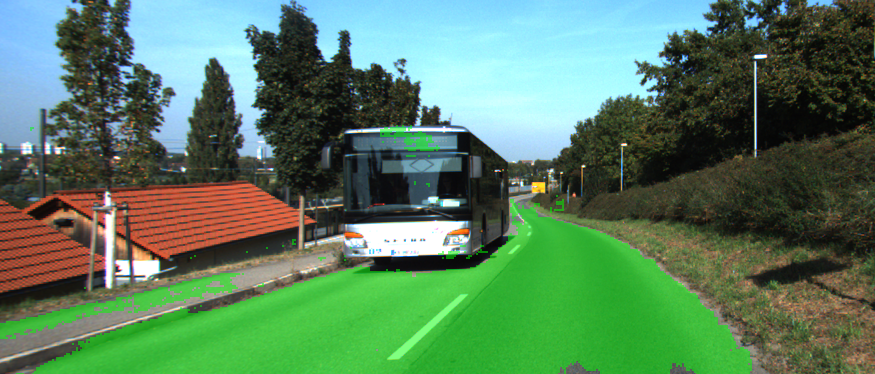
\includegraphics[width=\columnwidth]{figures/models/testing2-um_32_sliding_stride2.png}
    \caption{Using the sliding window approach with a stride of $s=2$.}%
\label{fig:stride2}
\end{figure}

The main disadvantage of this approach is the impractical runtime. For a
1~megapixel image we need to run 1~million classifications. This leads to a
runtime of almost two~minutes with our hardware. In order to reduce the
evaluation time we introduced an evaluation stride $s$. Similar to the training
stride we skip $s-1$ pixels in each dimension. This increases the evaluation
speed by a factor of $s^2$. For the sliding window approach we found that a
stride of $s = 10$ is a reasonable trade-off between speed and quality.
\Cref{fig:stride10} shows the result of the sliding window approach with a
stride of $s=10$.



\begin{figure}[H]
    \centering
    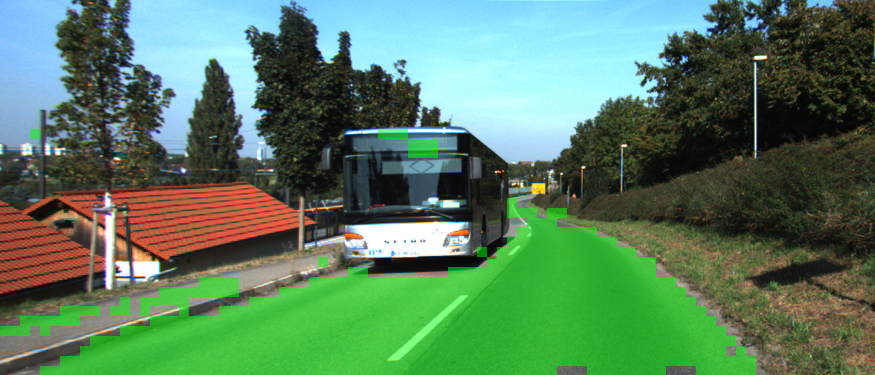
\includegraphics[width=\columnwidth]{figures/models/testing2-um_32_sliding_stride10.png}
    \caption{Using the sliding window approach with a stride of $s=10$.}%
\label{fig:stride10}
\end{figure}


\subsection{The Regression Approach}
The main disadvantage of our sliding window approach is that the segmentation
becomes very coarse with higher values for the stride $s$. To overcome this
problem we designed a regression neural networks which is able to classify each
pixel independently.

\subsubsection{Definition of the Regression Problem}
We trained a neural network to solve the following regression problem:

\fbox{
    \begin{tabular}{l l}
        \multicolumn{2}{l}{\textbf{Regression Problem}} \\
        \textit{Input:} & A $n \times n$ 3-channel pixel image section.\\
        \textit{Output:} & A $n \times n$ label.
    \end{tabular}
}

where the net is trained to minimize the mean squared error of the output. The
output of the regression net is continuous. We round the output to obtain a
binary classification. \Cref{fig:reg} visualizes our regression approach.

\begin{figure}[H]
    \centering
    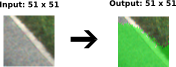
\includegraphics[width=0.5\columnwidth]{figures/models/fully-conv.png}
    \caption{Visualization of the regression approach.}%
\label{fig:reg}
\end{figure}

The goal is to choose $n$ as big as possible as $n^2$ is the number of pixels
which can be classified at once. However, due to GPU memory limitations we
cannot train a network with $n > 51$.


\subsubsection{Net Topology}
Similar to the classification approach our experiments show that a simple net
topologies work best. The topology we used is detailed in \cref{tab:topo2}.

\begin{savenotes}
\begin{table}[H]
    \normalsize
    \centering
    \begin{tabular}{r l l}
        \toprule
        \textbf{Layer} & \textbf{Type}  & \textbf{Shape}  \\
        \midrule
        0     & Input &  $51 \times 51 \times 3$ \\
        1     & Convolution & 10 filter  each $5 \times 5$ \\
        2     & Convolution & 1 filter $51 \times 51$  \\
        3     & Reshape (Flatten) & $51 \times 51$ \\
        4     & Output     & $2601\footnotemark \times 1$\\
        \bottomrule
    \end{tabular}
    \caption{Topology of the regression network.}%
\label{tab:topo2}
\end{table}
\footnotetext{The shape of $2601 \times 1$ is a result of flattening the $51 \times 51$ image patch. This is only necessary due to tooling support.}
\end{savenotes}


\subsubsection{Training}
Training of the regression model can be implemented analogously to the
classification model. We use overlapping image section again to get as much
information out of the data as possible.

\subsubsection{Evaluation}
In order to evaluate a whole image using the regression approach we divide the
image into patches of size $n \times n$ and evaluate each patch individually.
The output is shown in \cref{fig:reg_stride2}. The result is quite impressive,
especially regarding the overall runtime of about $\SI{0.18}{\second}$ as shown
in \cref{tab:runtime}.

\begin{figure}[]
    \centering
    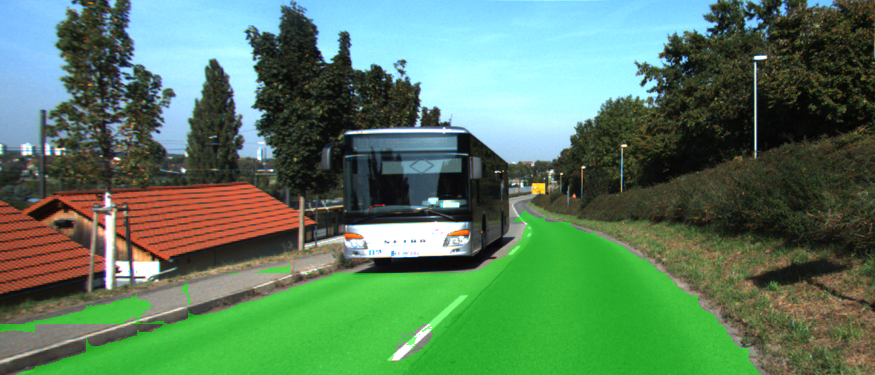
\includegraphics[width=\columnwidth]{figures/models/testing2-um_32_conv_stride51.png}
    \caption{Using regression approach with stride $s=51$}%
\label{fig:reg_stride2}
\end{figure}


One observation is, that the segmentation works better in the center of each
patch. The neural network does not have good information close to the border of
each image section. To overcome this problem we use an evaluation stride again.
This introduces an overlap between each image patch. A pixel $p$ is then
segmented according to the patch whose center is closer to $p$.


\begin{figure}[]
    \centering
    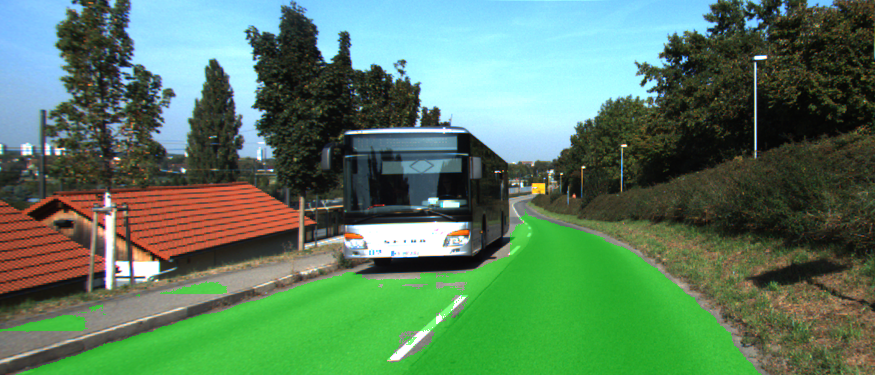
\includegraphics[width=\columnwidth]{figures/models/testing2-um_32_conv_stride37.png}
    \caption{Using regression approach with stride $s=37$}%
\label{fig:reg_stride37}
\end{figure}

\Cref{fig:reg_stride37} shows the output when using a stride of 37. We see that
the edge of the street is classified slightly better. In order to archive this
effect a rather big stride between 37~and~47 is already sufficient. In the
regression approach there is no measurable benefit of using strides below 37.
